\documentclass[paper=a4,fontsize=11pt,twocolumn,pagesize,bibtotoc]{scrartcl}

\usepackage[utf8]{inputenc}
\usepackage[T1]{fontenc}
\usepackage[english]{babel}

\usepackage[osf]{mathpazo}
\usepackage{microtype}
\usepackage{tikz}
\usetikzlibrary{automata}
\usepackage{amsthm, amssymb, amsmath}
\usepackage{graphicx}
\usepackage{color}
\usepackage{hyperref}

\parindent0pt


\usepackage{xr-hyper}

\usepackage{listings}

\lstset{   basicstyle=\ttfamily\scriptsize,
          breaklines=true
          }

\parindent0pt


\title{CMIDID documentation - alsa and gpio }
\subtitle{Linux Kernel Driver Implementation}
\author{Andreas R.}

\begin{document}
	\maketitle
	
This part of the documentation will provide information on the communication with the alsa sequencer and how it is implemented in the CMIDID driver. Also the setup of the raspberry pi is described to provide the right environment for using a  raspberry pi as an instrument.
\section{Raspberry Pi setup}
For this project the raspberry pi was chosen as hardware to develop and test the software. It is so small  that it could easily be used in a real instrument like an e-piano or an e-drum. Also it is has GPIO pins to connect test keys. The raspberry pi has 17 usable GPIO ports in the Rev. 2 board of the model B. With this, a maximum of 8 keys can be controlled by the board. In some scenarios this could be not enough, so either an additional connector must be used or another board with more GPIOs like the BeagleBone Black or the raspberry pi model B+.\\
Also the most important argument for the raspberry pi is the price which is very low for a full linux capable board. 
\\
The goal of the following section is to explain how the platform is set up to be used to develop on the device so that only a simple ssh client is needed.
\cite{gpiopins}
\section{raspbian}
There are a lot of different linux distributions available for the raspberry pi. For the CMIDID development raspbian was chosen because it is one of the most widely used distributions, it has a lot of packages available in its repository and it is easy to install. \\
To install raspbian, a computer is used to write the 800 MB image onto a sd card. After inserting the sd card into the raspberry pi the system starts up and can be used after a short setup. To compile and use the CMIDID driver the standard build utils like gcc, fluidsynth, alsa-utils, git have to be installed additionally. For further explanations it is assumed that the CMIDID project is checked out in the \texttt{/home/pi/CMIDID/} folder.
\section{linux sources and firmware manual}
One problem of raspbian is that there are no linux headers and sources available for the current kernel.
But as these are necessary for building a kernel module the linux sources can be downloaded from \url{https://github.com/raspberrypi/linux}. 
As the sources are very big also only the relevant sources until the version used for the compiled kernel can be used. For example by downloading a certain git hash or only a certain depth of commits.
Compiling the kernel on the raspberry pi takes very long so we need the symbol map of the compilation of the used kernel.
As \texttt{uname -a} prints the compiled kernel for example: \texttt{Linux raspberrypi 3.10.25+ \#622 PREEMPT Fri Jan 3 18:41:00 GMT 2014 armv6l GNU/Linux} the build number \texttt{\#622} can be extracted.
After downloading the firmware repository (\url{https://github.com/raspberrypi/firmware}) the git log has to be searched for \texttt{\#622} and choose the commit where the number was added.
With the git hash of this commit, the git repository is checked out to this state. After that in the file \texttt{extras/git\_hash} the hash for the linux repository can be found. Now the linux repositroy has to be checked out with this git hash. From the firmware repository the file\texttt{extra/Module.symvers} has to be copied to the build destination.\cite{linuxsrc}\\
After that a link should be created pointing from \texttt{/usr/lib/modules/`uname -r`/build/} to the linux repository. \\
After that the CMIDID project should compile by executing make in the folder \texttt{/home/pi/CMIDID/module}. 
The bash scripts \texttt{prepare\_module.sh} and \texttt{rewire\_module.sh} can be used to compile the module, start the software synthesizer and connect them.
 If the buttons are connected to the right GPIOs the keyboard should work otherwise the configuration can easily be changed.\\
If there is no sound after pressing the buttons it could be that the sound configuration is wrong which can be changed by the tool \texttt{raspi-config}
\subsection{alternatives}
There also exist scripts to do the things described in the previous section for example on \url{https://github.com/tz1/pikernomatic}. But there can always occur problems which can make it necessary to do it the manual way.\\
Another option would be to compile the module with cross compilation on a computer. Therefore every developer has to use a linux distribution and install another version of the gcc (\texttt{gcc-arm-linux-gnueabi}). This would decrease the compilation time which is quite high on the raspberry pi.
\section{ALSA}
\label{alsa}
ALSA, which stands for Advanced Linux Sound Architecture, was initially developed by Jaroslav Kysela as replacement for the OSS/Free audio/midi subsystem which had a lack of features and didn't support most of the new sound cards. Since kernel version 2.6 ALSA is the default sound system used by the kernel. The ALSA system has fully modularized sound drivers which means that new sound cards can be easily installed and be configured separately  by the user. Also it provides a user-space library called alsa-lib which makes it easy to run new sound programs as a normal user without changing the kernel.\\
ALSA can be configured with the command line tools alsaconf, alsamixer and alsactl. \\
Additionally to ALSA also JACK \cite{jack} could be used, which can make the process of synthesizing more accurate. In this scenario it was not used because it would increase the complexity of the setup and would probably bring no benefits in the standard use case.
\cite{Phillips:2005:UGA:1080072.1080075}
\subsection{midi api}
\begin{figure*}
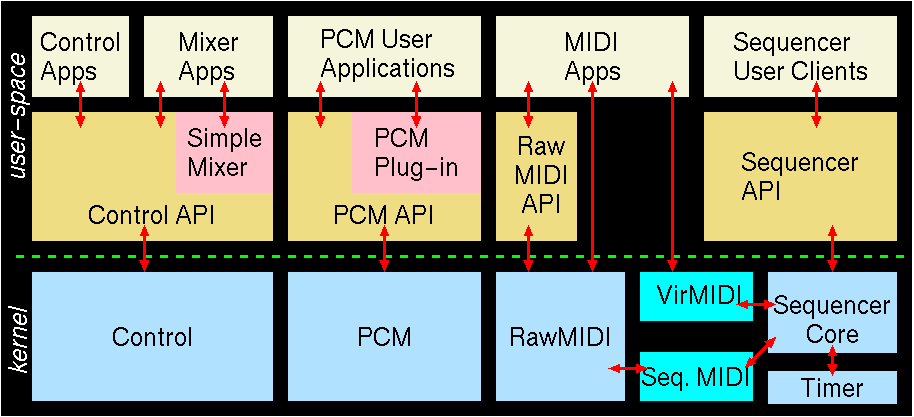
\includegraphics[keepaspectratio=true,width=\textwidth]{alsa.png}
\caption{ALSA Architecture from \url{http://www.alsa-project.org/~tiwai/lk2k/lk2k.html}}
\label{alsaarch}
\end{figure*}
There are different possibilities to communicate with the audio/midi system of linux. One possibility is over the \texttt{snd\_virmidi} module which is included in the stock kernel and can be simply loaded with \texttt{modprobe snd\_virmidi}. After that virtual midi devices are registered and also midi character devices are created for example: \texttt{/dev/snd/midiC2D0}. The ALSA virtual midi driver acts like a bridge between the internal ALSA midi sequencer and a raw midi stream. \\
Now a driver could create a character device itself to send out the midi events in a raw stream. This way has the advantage that it is very independent of the currently used API or sound system. Disadvantages of this data flow are that it is more complicated to configure as the \texttt{snd\_virmidi} module is always necessary and that we have a performance decrease because the raw data has to be encoded and decoded for the raw stream. The more direct way is to directly create an ALSA midi device and use the midi API. This method was used for the CMIDID driver. So the "Sequencer Core" of figure \ref{alsaarch} is the part which was directly used and the Sequencer API in the user-space what not used.
\subsection{midi initalization}
In the CMIDID driver the midi relevant code can be found in the file \texttt{module/CMIDID\_midi.c}. The initalization is called when the module is loaded and is implemented in the function \texttt{CMIDID\_midi\_init}.\\
First a normal sound card structure is created similar to drivers for physically attached sound cards: \begin{lstlisting}
snd_card_create(-1, NULL, THIS_MODULE ...
\end{lstlisting}
After that a sequencer client is attached to the created sound card. A real physical sound card can have a lot of different components like a midi sequencer or a line out. In the CMIDID driver the virtually created sound card consists only of a midi sequencer client with one port. For the initialization the created sound card is needed:
\begin{lstlisting}
state.client= snd_seq_create_kernel_client(state.card, 0, "CMIDID");
\end{lstlisting}
The client index 0 and the name "CMIDID" is later used to identify the sequencer. The saved \texttt{state.client} is important for later actions like sending out an event.\\ 
Now the sequencer must be configured. This can be done with userland ioctl or with the equivalent kernel space function.
\begin{lstlisting}
 snd_seq_kernel_client_ctl(state.client, SNDRV_SEQ_IOCTL_CREATE_PORT,&pinfo);
\end{lstlisting}
The command \texttt{SNDRV\_SEQ\_IOCTL\_CREATE\_PORT} creates a new midi port. In the port info struct \texttt{pinfo} information like the  capabilities of the port and the client id of the sequencer are stored.
\\
After loading the module the sequencer client should appear in \texttt{/proc/asound/seq/clients}. A sample output could look like this:
\begin{lstlisting}
Client  20 : "CMIDID" [Kernel]
  Port   0 : "port-0" (R-e-)
\end{lstlisting}
The client number depends on the clients already registered. In the driver it is the one saved in the \texttt{state.client} variable.
\subsection{midi event}
In the midi protocol consists of different small messages. In the raw format the messages take up to 3 bytes. The two commands used in the CMIDID driver are the 'note on event' and the 'note off event'. In the raw format the first bytes indicates which event it is and the channel on which the note should be turned on/off. The channel can be between 0 an 15 and identifies the instrument which should be used.
\\
The second byte is the key which was pressed and must be between 0 and 127. The synthesizer has a note assigned to every key so the key value can also be called as note.\\
 The third byte in the binary format describes the velocity with which the key was pressed. It can also be between 0 and 127. As the CMIDID driver does not use the raw format corresponding ALSA midi events have to be used.\\
As previously described the sequencer client has a port which can be used for communication. When a the key of the piano is pressed a midi event should be sent out.
This event is described by the \texttt{struct snd\_seq\_event}. This event is filled with information of the previously created client.  Also all the values used in the raw midi format can be put into the struct like type, note, velocity channel. Additionally it is important to tell ALSA how to deliver the the event:
\begin{lstlisting}
event->queue = SNDRV_SEQ_QUEUE_DIRECT;
event->dest.client = SNDRV_SEQ_ADDRESS_SUBSCRIBERS;
\end{lstlisting}
With these settings the event is delivered to all clients which were manually assigned to the CMIDID client. This can be configured from the userspace like described in
 \nameref{aconnect}.\\
 If the key is released a note off event is send out. It is important to send out a note off for every note on which was send out otherwise the synthesizer can show wrong behaviour. If somehow because of a network problem the driver does not remember the send out note on events it could alternatively send out an "Channel Mode Messages" with the command to set all notes off. This is currently not implemented.
\cite{midimessages}
\subsection{midi features}
When thinking of midi features the possibilities are nearly endless. Currently one midi feature is implemented to translate notes but other features could be easily added the same way. The translate ioctl call increments an internal variable. Now always when a new note is configured to be send out in the function \texttt{config\_note\_event} the saved value is added to the note.
\subsection{ALSA sequencer connection manager}
\label{aconnect}
The ALSA sequencer connection manager is a tool included in the alsa-utils which are available for all important linux distributions. With this command line tool it is possible to display all ports which where previously registered as input ports.
\begin{lstlisting}
>aconnect -i
	client 20: 'cmidid' [type=kernel]
		0 'port-0          '
\end{lstlisting}
If a \nameref{softwaresequencer} is started the port should be available in the aconnect output ports:
\begin{lstlisting}
>aconnect -o
	client 128: 'FLUID Synth (2274)' [type=user]
		0 'Synth input port (2274:0)'      '
\end{lstlisting}
In aconnect the input port is the sender which sends the midi events and the output port is the program which receives the midi events. The ports can be connected with a single aconnect call:
\begin{lstlisting}
	aconnect 20:0 128:00
\end{lstlisting}
The first pair describes the input client and its port and the second pair is the output client. Instead of the client ids also the names could be used.\\
To delete this connection the \texttt{-d} option can be used or with the \texttt{-x} option all connections are deleted. This is very important because if a client is connected the corresponding kernel module can not be unloaded. In this setup also more clients can be connect. For example if the applemidi module is loaded with another aconnect call the CMIDID client can additionally be connected to the applemidi client. Now every midi event is delivered to both clients. To avoid multi assignments the exclusive option \texttt{-e} can be used.
\subsection{software sequencer}
\label{softwaresequencer}
A software synthesizer is a program which simulates a hardware synthesizer and plays sounds like a normal instrument. There exists a wide range of software synthesizers reaching from expensive commercial software to open source projects. For the demonstration of the CMIDID driver the open source solution fluidsynth was used. Another option would have been the
TiMidity++ software synthesizer \url{http://timidity.sourceforge.net/} which is also open source and offers a gui, which is not helpful for the this scenario.
\\
Fluidsynth is a command line tool using the SoundFont 2 specification and is available for Linux, Windows and Mac OSX. To use the tool a soundfont is necessary, which can be found online for different instruments. With the channel it is possible to specify the instrument. The software can be started as server in the background with a simple command:
\begin{lstlisting}
fluidsynth -is -a alsa /PATH/TO/SOUNDFONT.sf2
\end{lstlisting}
There are a lot of more options available for fluidsynth which could sometimes be necessary to avoid noise on the output. Also it can help to execute it with root privileges.
\cite{fluidsynth}

\bibliographystyle{alpha}
\bibliography{sources}
	
	
\end{document}